\documentclass[12pt,twoside]{ctexart}
\usepackage{geometry}
\geometry{left=2.5cm,right=2.5cm,top=1.2cm,bottom=1cm}
\renewcommand{\baselinestretch}{1.5} \normalsize%:不改变字体大小,只改变行距。
\usepackage{examanswersheetv2,caption2,pifont,ulem}
%\mifengxian
\begin{document}
%电脑上需要安装相应字体,分别是方正小标宋和楷体
%
%	试卷标题
%
\begin{center}

\zihao{-2}{高$2016$级高二上期周练(二)}
\end{center}

%\zongfenlana

%
%	试卷正面
%
\begin{enumerate}
\item[\kaishu{}一]{\kaishu{}选择题,共六题}%-------------------------------------选择题
\item 圆$2x^2+2y^2-4ax+12ay+16a^2=0(a<0)$的周长等于
\xxs{2\sqrt{2}a}{-2\sqrt{2}a}{2a^2\pi}{-2\sqrt{2}a\pi}

\item 已知直线$ax+by+c=0(abc\neq 0)$与圆$x^2+y^2=1$相切,则三条边长分别为$|a|,|b|,|c|$的三角形是
\xx{锐角三角形}{直角三角形}{钝角三角形}{不存在}

\item 函数$f(x)$在$(-\infty,+\infty)$单调递减,且为奇函数.若$f(1)=-1$,则满足$-1\leq f(x-2)\leq 1$的$x$的取值范围是
\xxs{[-2,2]}{[-1,1]}{[0,4]}{[1,3]} 

\item 若实数$x,y$满足$x^2+y^2+4x-2y-4=0$,则$\sqrt{x^2+y^2}$的最大值是
\xxs{\sqrt{5}+3}{\sqrt{5}+14}{-\sqrt{5}+3}{-\sqrt{5}+14}

\item 已知集合$M=\{(x,y)|y=\sqrt{9-x^2},y\neq 0\},N=\{(x,y)|y=x+b\}$,若$M\cap N\neq \varnothing$,则实数$b$的取值范围是
\xxs{[-3\sqrt{2},3\sqrt{2}]}
{[-3,3]}
{(-3,3\sqrt{2}]}
{[-3\sqrt{2},3)}

\item 设函数$f(x)=\left\{
\begin{aligned}
	1-|x-1| &,&x\in (-\infty,2)\\
	\dfrac{1}{2}f(x-2) &,&x\in [2,+\infty)
\end{aligned}\right.$,则函数$g(x)=xf(x)-1$的零点个数为~~~\hfill
\xxs{4}{5}{6}{7} 

\item[\kaishu{}二]{\kaishu{}填空题,共三题}%--------------------------------------填空题


\item 已知$P(3,0)$为圆$C:x^2+y^2-8x-2y+12=0$内一点,则过$P$点的最短弦所在直线方程是\line{2},过$P$点的最长弦所在直线方程是\line{2}.


\item 经过$A(6,5),B(0,1)$两点,且圆心在直线$3x+10y+9=0$上的圆的方程是\line{2}

\item 已知$a\in \mathbf{R}$,函数$f(x)=|x+\dfrac{4}{x}-a|+a$,在区间$[1,4]$上的最大值是$5$,则$a$的取值范围是\line{2}.
\begin{center}
	\begin{tabular}{|p{1.5cm}|p{1.5cm}|p{1.5cm}|p{1.5cm}|p{1.5cm}|p{1.5cm}|p{1.5cm}|}
	\hline
	题号 &1&2 &3 &4 &5 &6  \\
	\hline
	答案 &D &B &D &A &C &C  \\
	\hline
		
	\end{tabular}
\end{center}

7.\underline{$x+y-3=0$},\underline{$x-y-3=0$} \hfill 8.\underline{$(x-7)^2+(y+3)^2=65$} \hfill 9.\underline{$(-\infty,\frac{9}{2}]$}

\item[\kaishu{}三]{\kaishu{}解答题,共四题}%-----------------------------------------------解答题

\item 已知函数$f(x)=\sin ^2 x-\cos ^2 x-2\sqrt{3}\sin x \cos x(x \in \mathbf{R}).$\\
(1)求$f(\dfrac{2\pi}{3})$的值;\\
(2)求$f(x)$的最小正周期及单调递增区间.\\
解:(1)因为$f(x)=\sin ^2 x-\cos ^2 x-2\sqrt{3}\sin x \cos x=-\cos 2x -\sqrt{3}\sin 2x=-2\sin (2x+\dfrac{\pi}{6})$,\\
所以$f(\dfrac{2\pi}{3})=-2\sin \dfrac{3\pi}{2}=2;$\\
(2)由(1)得$f(x)$的最小正周期为$\pi$,\\
令$\dfrac{\pi}{2}+2k\pi \leq 2x+\dfrac{\pi}{6}\leq \dfrac{3\pi}{2}+2k\pi ~~(k \in \mathbb{Z})$,\\
解得$f(x)$的单调递增区间为$[\dfrac{\pi}{6}+k\pi,\dfrac{2\pi}{3}+k\pi]~~(k \in \mathbb{Z})$.



\item 已知点$M(3,1)$,直线$ax-y+4=0$及圆$C:(x-1)^2+(y-2)^2=4$.\\
(1)求过$M$点的圆$C$的切线方程;\\
(2)若直线$ax-y+4=0$与圆$C$相切,求$a$的值;\\
(3)若直线$ax-y+4=0$与圆$C$相交于$A,B$两点,且弦$AB$的长为$2\sqrt{3}$,求$a$的值;
解:(1)因为$(3-1)^2+(1-2)^2>4$,\\
所以点$M$在圆$(x-1)^2+(y-2)^2=4$外,\\
当斜率不存在时,$x=3$满足与圆$C$相切,\\
当斜率存在时,设切线方程为$y-1=k(x-3)$,即$kx-y-3k+1=0$,\\
由$\dfrac{|k-2+1-3k|}{\sqrt{k^2+1}}=2$,得$k=\dfrac{3}{4}$.\\
故所求的切线方程为$x=3$或$3x-4y-5=0$.\\
(2)由直线$ax-y+4=0$与圆$C$相切,\\
所以$\dfrac{|a-2+4|}{\sqrt{1+a^2}}=2$,解得$a=0$或$a=\dfrac{4}{3}$.\\
(3)圆心到直线的距离$d=\dfrac{|a+2|}{\sqrt{1+a^2}}$,弦长$L=2\sqrt{3},r=2,$\\
由$r^2=d^2+(\dfrac{L}{2})^2$,得$a=-\dfrac{3}{4}$.


%
%	试卷背面
%


\item 如图所示,等腰梯形$ABCD$的底边$AB$在$x$轴上,顶点$A$与顶点$B$关于原点$O$对称,且底边$AB$和$CD$的长分别为$6$和$2\sqrt{6}$,高为$3$.\\
(1)求等腰梯形$ABCD$的外接圆$E$的方程;\\
(2)若点$N$的坐标为$(5,2)$,点$M$在圆$E$上运动,求线段$MN$的中点$P$的轨迹方程.
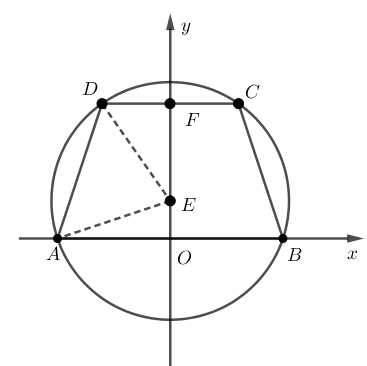
\includegraphics[width=4cm,height=4cm]{121.png}\\
解:(1)连接$AE,DE,$设圆的半径为$r$,设$CD$与$y$轴交于点$F$,\\
$EF=\sqrt{r^2-6},OE=\sqrt{r^2-9},\sqrt{r^2-6}+\sqrt{r^2-9}=3,$\\
解得$r=\sqrt{10},$所以$OE=1$,\\
所以圆$E$的方程为$x^2+(y-1)^2=10$.\\
(2)设$P(x,y),M(2x-5,2y-2)$,因为点$M$在圆上运动,所以可把$M$代入圆的方程中,得:\\
$(2x-5)^2+(2y-3)^2=10$即$x^2+y^2-5x-3y+6=0$.\\
故$P$的轨迹方程为$x^2+y^2-5x-3y+6=0$.




\item (选做题)已知直线$l_1:mx-y=0,l_2:x+my-m-2=0$.\\
(1)求证:对任意的实数$m,l_1$和$l_2$的交点$M$总在一个定圆上;\\
(2)若$l_1$与(1)中定圆的另一个交点为$P_1,l_2$与(1)中定圆的另一个交点为$P_2$,求当实数$m$取值变化,$\triangle MP_1P_2$的面积取最大值时,直线$l_1$的方程.

证明:(1)由题意可得$$\left \{ \begin{aligned}
	mx-y & =&0 \\
	x+my-m-2 &= &0
\end{aligned}\right.$$
消去$m$可得$x^2+y^2-2x-y=0$.方程表示一个以$(1,\dfrac{1}{2})$为圆心,$\dfrac{\sqrt{5}}{2}$为半径的圆,故得证.\\
(2)由题可知,直线$l_1,l_2$分别恒过定点$(0,0),(2,1)$,并且两定点都在圆上,\\
故$P_1(0,0),P_2(2,1)$\\
因为$P_1P_2$是圆$C$的直径,\\
当且仅当圆心$C(1,\dfrac{1}{2})$到$l_1$的距离等于$C$到$l_2$的距离时,$\triangle MP_1P_2$的面积取最大值,\\
所以$$\dfrac{|m-\dfrac{1}{2}|}{\sqrt{m^2+1}}=\dfrac{|\dfrac{1}{2}m+1|}{\sqrt{m^2+1}}$$
解得:$m=3$或$m=-\dfrac{1}{3},$\\
所以直线$l_1$的方程为$3x-y=0$或$x+3y=0.$




% \newpage
\end{enumerate}
\end{document}